\documentclass{ximera}

%\usepackage{todonotes}
%\usepackage{mathtools} %% Required for wide table Curl and Greens
%\usepackage{cuted} %% Required for wide table Curl and Greens
\newcommand{\todo}{}

\usepackage{multicol}

\usepackage{esint} % for \oiint
\ifxake%%https://math.meta.stackexchange.com/questions/9973/how-do-you-render-a-closed-surface-double-integral
\renewcommand{\oiint}{{\large\bigcirc}\kern-1.56em\iint}
\fi

\graphicspath{
  {./}
  {ximeraTutorial/}
  {basicPhilosophy/}
  {functionsOfSeveralVariables/}
  {normalVectors/}
  {lagrangeMultipliers/}
  {vectorFields/}
  {greensTheorem/}
  {shapeOfThingsToCome/}
  {dotProducts/}
  {partialDerivativesAndTheGradientVector/}
  {../ximeraTutorial/}
  {../productAndQuotientRules/exercises/}
  {../motionAndPathsInSpace/exercises/}
  {../normalVectors/exercisesParametricPlots/}
  {../continuityOfFunctionsOfSeveralVariables/exercises/}
  {../partialDerivativesAndTheGradientVector/exercises/}
  {../directionalDerivativeAndChainRule/exercises/}
  {../commonCoordinates/exercisesCylindricalCoordinates/}
  {../commonCoordinates/exercisesSphericalCoordinates/}
  {../greensTheorem/exercisesCurlAndLineIntegrals/}
  {../greensTheorem/exercisesDivergenceAndLineIntegrals/}
  {../shapeOfThingsToCome/exercisesDivergenceTheorem/}
  {../greensTheorem/}
  {../shapeOfThingsToCome/}
  {../separableDifferentialEquations/exercises/}
  {../dotproducts/}
  {../functionsOfSeveralVariables/}
  {../lagrangeMultipliers/}
  {../partialDerivativesAndTheGradientVector/}
  {../normalVectors/}
  {../vectorFields/}
}
\def\xmNotExpandableAsAccordion{true}

\newcommand{\mooculus}{\textsf{\textbf{MOOC}\textnormal{\textsf{ULUS}}}}

\usepackage{tkz-euclide}\usepackage{tikz}
\usepackage{tikz-cd}
\usetikzlibrary{arrows}
\tikzset{>=stealth,commutative diagrams/.cd,
  arrow style=tikz,diagrams={>=stealth}} %% cool arrow head
\tikzset{shorten <>/.style={ shorten >=#1, shorten <=#1 } } %% allows shorter vectors

\usetikzlibrary{backgrounds} %% for boxes around graphs
\usetikzlibrary{shapes,positioning}  %% Clouds and stars
\usetikzlibrary{matrix} %% for matrix
\usepgfplotslibrary{polar} %% for polar plots
\usepgfplotslibrary{fillbetween} %% to shade area between curves in TikZ
%\usetkzobj{all} %% obsolete

\usepackage[makeroom]{cancel} %% for strike outs
%\usepackage{mathtools} %% for pretty underbrace % Breaks Ximera
%\usepackage{multicol}
\usepackage{pgffor} %% required for integral for loops

\usepackage{tkz-tab}  %% for sign charts

%% http://tex.stackexchange.com/questions/66490/drawing-a-tikz-arc-specifying-the-center
%% Draws beach ball
\tikzset{pics/carc/.style args={#1:#2:#3}{code={\draw[pic actions] (#1:#3) arc(#1:#2:#3);}}}



\usepackage{array}
\setlength{\extrarowheight}{+.1cm}
\newdimen\digitwidth
\settowidth\digitwidth{9}
\def\divrule#1#2{
\noalign{\moveright#1\digitwidth
\vbox{\hrule width#2\digitwidth}}}





\newcommand{\RR}{\mathbb R}
\newcommand{\R}{\mathbb R}
\newcommand{\N}{\mathbb N}
\newcommand{\Z}{\mathbb Z}

\newcommand{\sagemath}{\textsf{SageMath}}


\renewcommand{\d}{\,d}
%\def\d{\mathop{}\!d}
%\def\d{\,d}

\AddToHook{begindocument}{%
  \renewcommand{\d}{\,d}     % lualatex redefines \d to underdot !!!
}

\pgfplotsset{
    every axis/.style={
        scale only axis,
        enlargelimits=false,
        trim axis left,
        trim axis right,
        clip=true,
    }
}

\newcommand{\dd}[2][]{\frac{\d #1}{\d #2}}
\newcommand{\pp}[2][]{\frac{\partial #1}{\partial #2}}
\renewcommand{\l}{\ell}
\newcommand{\ddx}{\frac{d}{\d x}}

\newcommand{\zeroOverZero}{\ensuremath{\boldsymbol{\tfrac{0}{0}}}}
\newcommand{\inftyOverInfty}{\ensuremath{\boldsymbol{\tfrac{\infty}{\infty}}}}
\newcommand{\zeroOverInfty}{\ensuremath{\boldsymbol{\tfrac{0}{\infty}}}}
\newcommand{\zeroTimesInfty}{\ensuremath{\small\boldsymbol{0\cdot \infty}}}
\newcommand{\inftyMinusInfty}{\ensuremath{\small\boldsymbol{\infty - \infty}}}
\newcommand{\oneToInfty}{\ensuremath{\boldsymbol{1^\infty}}}
\newcommand{\zeroToZero}{\ensuremath{\boldsymbol{0^0}}}
\newcommand{\inftyToZero}{\ensuremath{\boldsymbol{\infty^0}}}



\newcommand{\numOverZero}{\ensuremath{\boldsymbol{\tfrac{\#}{0}}}}
\newcommand{\dfn}{\textbf}
%\newcommand{\unit}{\,\mathrm}
\newcommand{\unit}{\mathop{}\!\mathrm}
\newcommand{\eval}[1]{\bigg[ #1 \bigg]}
\newcommand{\seq}[1]{\left( #1 \right)}
\renewcommand{\epsilon}{\varepsilon}
\renewcommand{\phi}{\varphi}


\renewcommand{\iff}{\Leftrightarrow}

\DeclareMathOperator{\arccot}{arccot}
\DeclareMathOperator{\arcsec}{arcsec}
\DeclareMathOperator{\arccsc}{arccsc}
\DeclareMathOperator{\si}{Si}
\DeclareMathOperator{\scal}{scal}
\DeclareMathOperator{\sign}{sign}


%% \newcommand{\tightoverset}[2]{% for arrow vec
%%   \mathop{#2}\limits^{\vbox to -.5ex{\kern-0.75ex\hbox{$#1$}\vss}}}
\newcommand{\arrowvec}[1]{{\overset{\rightharpoonup}{#1}}}
%\renewcommand{\vec}[1]{\arrowvec{\mathbf{#1}}}
\renewcommand{\vec}[1]{{\overset{\boldsymbol{\rightharpoonup}}{\mathbf{#1}}}\hspace{0in}}

\newcommand{\point}[1]{\left(#1\right)} %this allows \vector{ to be changed to \vector{ with a quick find and replace
\newcommand{\pt}[1]{\mathbf{#1}} %this allows \vec{ to be changed to \vec{ with a quick find and replace
\newcommand{\Lim}[2]{\lim_{\point{#1} \to \point{#2}}} %Bart, I changed this to point since I want to use it.  It runs through both of the exercise and exerciseE files in limits section, which is why it was in each document to start with.

\DeclareMathOperator{\proj}{\mathbf{proj}}
\newcommand{\veci}{{\boldsymbol{\hat{\imath}}}}
\newcommand{\vecj}{{\boldsymbol{\hat{\jmath}}}}
\newcommand{\veck}{{\boldsymbol{\hat{k}}}}
\newcommand{\vecl}{\vec{\boldsymbol{\l}}}
\newcommand{\uvec}[1]{\mathbf{\hat{#1}}}
\newcommand{\utan}{\mathbf{\hat{t}}}
\newcommand{\unormal}{\mathbf{\hat{n}}}
\newcommand{\ubinormal}{\mathbf{\hat{b}}}

\newcommand{\dotp}{\bullet}
\newcommand{\cross}{\boldsymbol\times}
\newcommand{\grad}{\boldsymbol\nabla}
\newcommand{\divergence}{\grad\dotp}
\newcommand{\curl}{\grad\cross}
%\DeclareMathOperator{\divergence}{divergence}
%\DeclareMathOperator{\curl}[1]{\grad\cross #1}
\newcommand{\lto}{\mathop{\longrightarrow\,}\limits}

\renewcommand{\bar}{\overline}

\colorlet{textColor}{black}
\colorlet{background}{white}
\colorlet{penColor}{blue!50!black} % Color of a curve in a plot
\colorlet{penColor2}{red!50!black}% Color of a curve in a plot
\colorlet{penColor3}{red!50!blue} % Color of a curve in a plot
\colorlet{penColor4}{green!50!black} % Color of a curve in a plot
\colorlet{penColor5}{orange!80!black} % Color of a curve in a plot
\colorlet{penColor6}{yellow!70!black} % Color of a curve in a plot
\colorlet{fill1}{penColor!20} % Color of fill in a plot
\colorlet{fill2}{penColor2!20} % Color of fill in a plot
\colorlet{fillp}{fill1} % Color of positive area
\colorlet{filln}{penColor2!20} % Color of negative area
\colorlet{fill3}{penColor3!20} % Fill
\colorlet{fill4}{penColor4!20} % Fill
\colorlet{fill5}{penColor5!20} % Fill
\colorlet{gridColor}{gray!50} % Color of grid in a plot

\newcommand{\surfaceColor}{violet}
\newcommand{\surfaceColorTwo}{redyellow}
\newcommand{\sliceColor}{greenyellow}




\pgfmathdeclarefunction{gauss}{2}{% gives gaussian
  \pgfmathparse{1/(#2*sqrt(2*pi))*exp(-((x-#1)^2)/(2*#2^2))}%
}


%%%%%%%%%%%%%
%% Vectors
%%%%%%%%%%%%%

%% Simple horiz vectors
\renewcommand{\vector}[1]{\left\langle #1\right\rangle}


%% %% Complex Horiz Vectors with angle brackets
%% \makeatletter
%% \renewcommand{\vector}[2][ , ]{\left\langle%
%%   \def\nextitem{\def\nextitem{#1}}%
%%   \@for \el:=#2\do{\nextitem\el}\right\rangle%
%% }
%% \makeatother

%% %% Vertical Vectors
%% \def\vector#1{\begin{bmatrix}\vecListA#1,,\end{bmatrix}}
%% \def\vecListA#1,{\if,#1,\else #1\cr \expandafter \vecListA \fi}

%%%%%%%%%%%%%
%% End of vectors
%%%%%%%%%%%%%

%\newcommand{\fullwidth}{}
%\newcommand{\normalwidth}{}



%% makes a snazzy t-chart for evaluating functions
%\newenvironment{tchart}{\rowcolors{2}{}{background!90!textColor}\array}{\endarray}

%%This is to help with formatting on future title pages.
\newenvironment{sectionOutcomes}{}{}



%% Flowchart stuff
%\tikzstyle{startstop} = [rectangle, rounded corners, minimum width=3cm, minimum height=1cm,text centered, draw=black]
%\tikzstyle{question} = [rectangle, minimum width=3cm, minimum height=1cm, text centered, draw=black]
%\tikzstyle{decision} = [trapezium, trapezium left angle=70, trapezium right angle=110, minimum width=3cm, minimum height=1cm, text centered, draw=black]
%\tikzstyle{question} = [rectangle, rounded corners, minimum width=3cm, minimum height=1cm,text centered, draw=black]
%\tikzstyle{process} = [rectangle, minimum width=3cm, minimum height=1cm, text centered, draw=black]
%\tikzstyle{decision} = [trapezium, trapezium left angle=70, trapezium right angle=110, minimum width=3cm, minimum height=1cm, text centered, draw=black]


\outcome{Estimate partial derivatives from tables and graphs.}

\author{Jim Talamo}
% The contour plots were produced with the following Maple Commands

%with(plots);
%p := contourplot(4/((x-1)^2+(y-2)^2)-4/((x+3)^2+(y-1)^2)+6/(x^2+(y+2)^2), x = -4.5 .. 4.5, y = -4.5 .. 4.5, contours = [-3, -1, -1/2, 0, 1/2, 1, 1.5, 5], grid = [100, 100]);

%I will look into exporting the data from the plot to draw this in TikZ later

%Plan: I will ask this same question AFTER they learn about the properties of the gradient

\begin{document}
\begin{exercise}

This exercise gives an example of an important type of contour plot that arises in electrostatics.

The magnitude of force that a particle of charge $Q$ exerts on a particle of charge $q$ that is $r$ units away is given by \emph{Coulomb's Law}

\[
F(r) = \frac{kQq}{r^2},
\] 

where $k =8.99 \times 10^9\unit{N}\cdot\unit{m}^2 /\unit{C}^2$ is Coulomb's constant.

When several charges are placed near each other, the force that a test particle of charge $q$ experiences is determined by adding the forces that each charged particle exerts on it.  The \emph{electric field} is a ``vector field''; to each point $(x,y)$ in the $xy$-plane, the electric field associates the force vector experienced by the test charge $q$.

An interesting fact is that this electric field can actually be realized as the gradient of a certain function $V(x,y)$, called the \emph{electric potential} via the formula

\[
\vec{E}(x,y)=-\grad{V}(x,y),
\]
and a useful way to visualize electric fields to plot the level curves of the electric potential.  These level curves are often referred to as \emph{equipotential lines}.

The contour plot for the electric potential $V(x,y)$ are below shows equipotential lines for an electric field that results from a charge configuration with positive charges at $(1,2)$ and $(0,-2)$ and a negative charge at $(-3,1)$.

\begin{image}
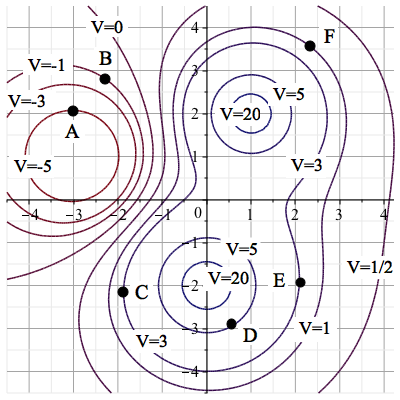
\includegraphics[width=5in]{contours3.png}
\end{image}
Assume $V(x,y)$ either increases or decreases between contour lines and $V_x(x,y)$ and $V_y(x,y)$ are defined at all points in the picture.

Select all of the points where $V_x(x,y)=0$.

\begin{selectAll}
\choice[correct]{A}
\choice{B}
\choice{C}
\choice{D}
\choice{E}
\choice{F}
\end{selectAll}

\begin{hint}
Note that the contour plot shows the level curves of the function $V(x,y)$ in the $xy$-plane, and gives the value that the function takes along them.  For instance, the points $C$, $E$, and $F$ lie along the level curve associated to $V=3$.

An important observation is the following.

\begin{quote}
Since the values of a function do not change along a level curve, the tangent line to a level curve gives the direction in which the instantaneous rate of change of the function is $0$.
\end{quote}

$V_x(a,b)$ is the instantaneous rate of change of the function at $(a,b)$ in the $x$-direction.  Thus, to find the points at which $V_x=0$, we need to look for the locations where the tangent line to the level curve is in the $x$-direction.  This occurs at point $A$ only.

\end{hint}

%%%%%%%%%%%%%%%%%%%%%%%%%%%%%%%%%%%%%%%%%%%%%%%%%%%%%%
\begin{exercise}
Select all of the points where $V_y(x,y)=0$.

\begin{selectAll}
\choice{A}
\choice{B}
\choice[correct]{C}
\choice{D}
\choice[correct]{E}
\choice{F}
\end{selectAll}

\end{exercise}  
%%%%%%%%%%%%%%%%%%%%%%%%%%%%%%%%%%%%%%%%%%%%%%%%%%%%%%
\begin{exercise}
Select all of the points where $V_x(x,y)>0$.

\begin{selectAll}
\choice{A}
\choice[correct]{B}
\choice[correct]{C}
\choice{D}
\choice{E}
\choice{F}
\end{selectAll}

\begin{hint}
To find where $V_x>0$, we need to look for when the function increases in the $x$-direction.  Since the function either must increase or must decrease between contours, note

\begin{itemize}
\item We've already determined that $V_x =0$ at point $A$.
\item 
As $x$ increases from point $B$, we move from the contour curve along which $V=-1$ towards the one where $V=0$.  Thus, $V_x>0$ at $B$.
\item As $x$ increases from point $C$, we move from the contour curve along which $V=\answer{3}$ towards the one where $V=\answer{5}$.  Thus, \wordChoice{\choice{$V_x<0$}\choice{$V_x=0$}\choice[correct]{$V_x>0$}} at  $C$.
\item As $x$ increases from point $D$, we move from the contour curve along which $V=\answer{5}$ towards the one where $V=\answer{3}$.  Thus, \wordChoice{\choice[correct]{$V_x<0$}\choice{$V_x=0$}\choice{$V_x>0$}} at  $D$.
\end{itemize}

\end{hint}
\end{exercise}  
%%%%%%%%%%%%%%%%%%%%%%%%%%%%%%%%%%%%%%%%%%%%%%%%%%%%%%
\begin{exercise}
Select all of the points where $V_y(x,y)<0$.

\begin{selectAll}
\choice{A}
\choice{B}
\choice{C}
\choice{D}
\choice{E}
\choice[correct]{F}
\end{selectAll}

\end{exercise}  

\end{exercise}
\end{document}
